\chapter{Project Architecture and Design}

In the following text, the author will describe the architecture and design of the Thesis Management System including functional, non-functional requirements and the domain model. The author will also depict some design parts with UML\footnote{Unified Modeling Language} 2.0 diagrams, however, the UML diagrams are not to be regarded as blueprints of the system but rather as sketches and as such, some information that the author considers irrelevant or obvious could be let out. This is allowed as stated by Martin Fowler in his book UML Distilled\cite{fowler-uml}.

\section{Functional Requirements}

\begin{enumerate}
    \item User management\\
    The system allows to create, read, update and delete (CRUD) users. User contains fields full name, email and password.

    \item Registration\\
    Anonymous users can sign up only with emails hosted at configured domain addresses.

    \item Log In\\
    Anonymous users can sign in using email and password.

    \item Site configuration\\
    Administrator can configure certain aspects of the system, like allowed email domain addresses, site announcement and the terms of use.

    \item Thesis topic management\\
    The system allows to CRUD thesis topics. Topic contains fields title and description in two languages.

    \item Category management\\
    The system allows to CRUD categories. Category contains fields title and description.

    \item Thesis topic can be added to categories.\\
    Topics can be added to one or more categories which allows users to browse topics in categories.

    \item Tags can be assigned to thesis topics\\
    There can be zero or more tags assigned to one thesis topic.

    \item Thesis topic contains field for a leader\\
    The leader has the authority to manage thesis topics created by them.

    \item University management\\
    The system allows to CRUD universities. University contains a field for the name of the university.

    \item Thesis topic contains field for the list of universities\\
    This field contains the list of universities that the topic is offered to. One thesis topic can be offered to one or more universities.

    \item Thesis topic contains field for the list of supervisors\\
    This field contains the list of university supervisors, each supervisor is assigned a university that they supervise at. Thesis topic can have zero or more university supervisors.

    \item Thesis topic contains field for the list of types\\
    This field contains the list of types (i.e. diploma, bachelor). Thesis topic can have zero or more types.

    \item Application management\\
    The system allows to CRUD applications.

    \item Students can apply for a thesis topic\\
    The applicant chooses the type and the university that they apply to.

    \item Applications can be approved\\
    To approve an application, the leader or a supervisor must create a new thesis.

    \item Thesis topic can be enabled or disabled

    \item Thesis topics can be filtered\\
    The system allows to filter thesis topics by university, type, leader or title.

    \item Thesis management\\
    The system allows to CRUD theses. Thesis contains fields title, description, thesis topic, assignee, supervisor, abstract, type and university.

    \item Tags can be assigned to theses\\
    There can be zero or more tags assigned to one thesis.

    \item Thesis contains field status\\
    Status can be either `in progress', `finished', `failed' or `postponed'.

    \item Thesis contains field grade\\
    One of A, B, C, D, E or F.

    \item Supervisor can select universities they supervise at for each thesis topic

    \item Supervisor can add private notes to theses

    \item Authenticated user can subscribe for thesis topics and theses\\
    The system sends notifications to all subscribers of a thesis topic or a thesis when a change is made to it.

    \item Authenticated user can unsubscribe from thesis topics and theses

    \item Theses can be filtered\\
    The system allows to filter theses by title, supervisor, assignee, status, grade, type or university.

    \item Theses and thesis topics can be filtered by tags\\
    The system allows to list theses or thesis topics that contains a particular tag.

    \item File management for theses\\
    The system allows to upload files to theses.

    \item Discussion for thesis topics and theses\\
    Logged in users can comment on thesis topics and theses.

    \item Private comments\\
    Users with certain authority can create comments that are not visible to students and guests.

    \item Full text search\\
    Theses and thesis topics can be searched by a full text search engine.

    \item Frequently Asked Questions (FAQ) management\\
    The system allows to CRUD Frequently Asked Questions. One frequently asked question contains fields question, answer and locale.

\end{enumerate}

\subsection{Use Case Diagram}

\begin{figure}[H]
    \centering
        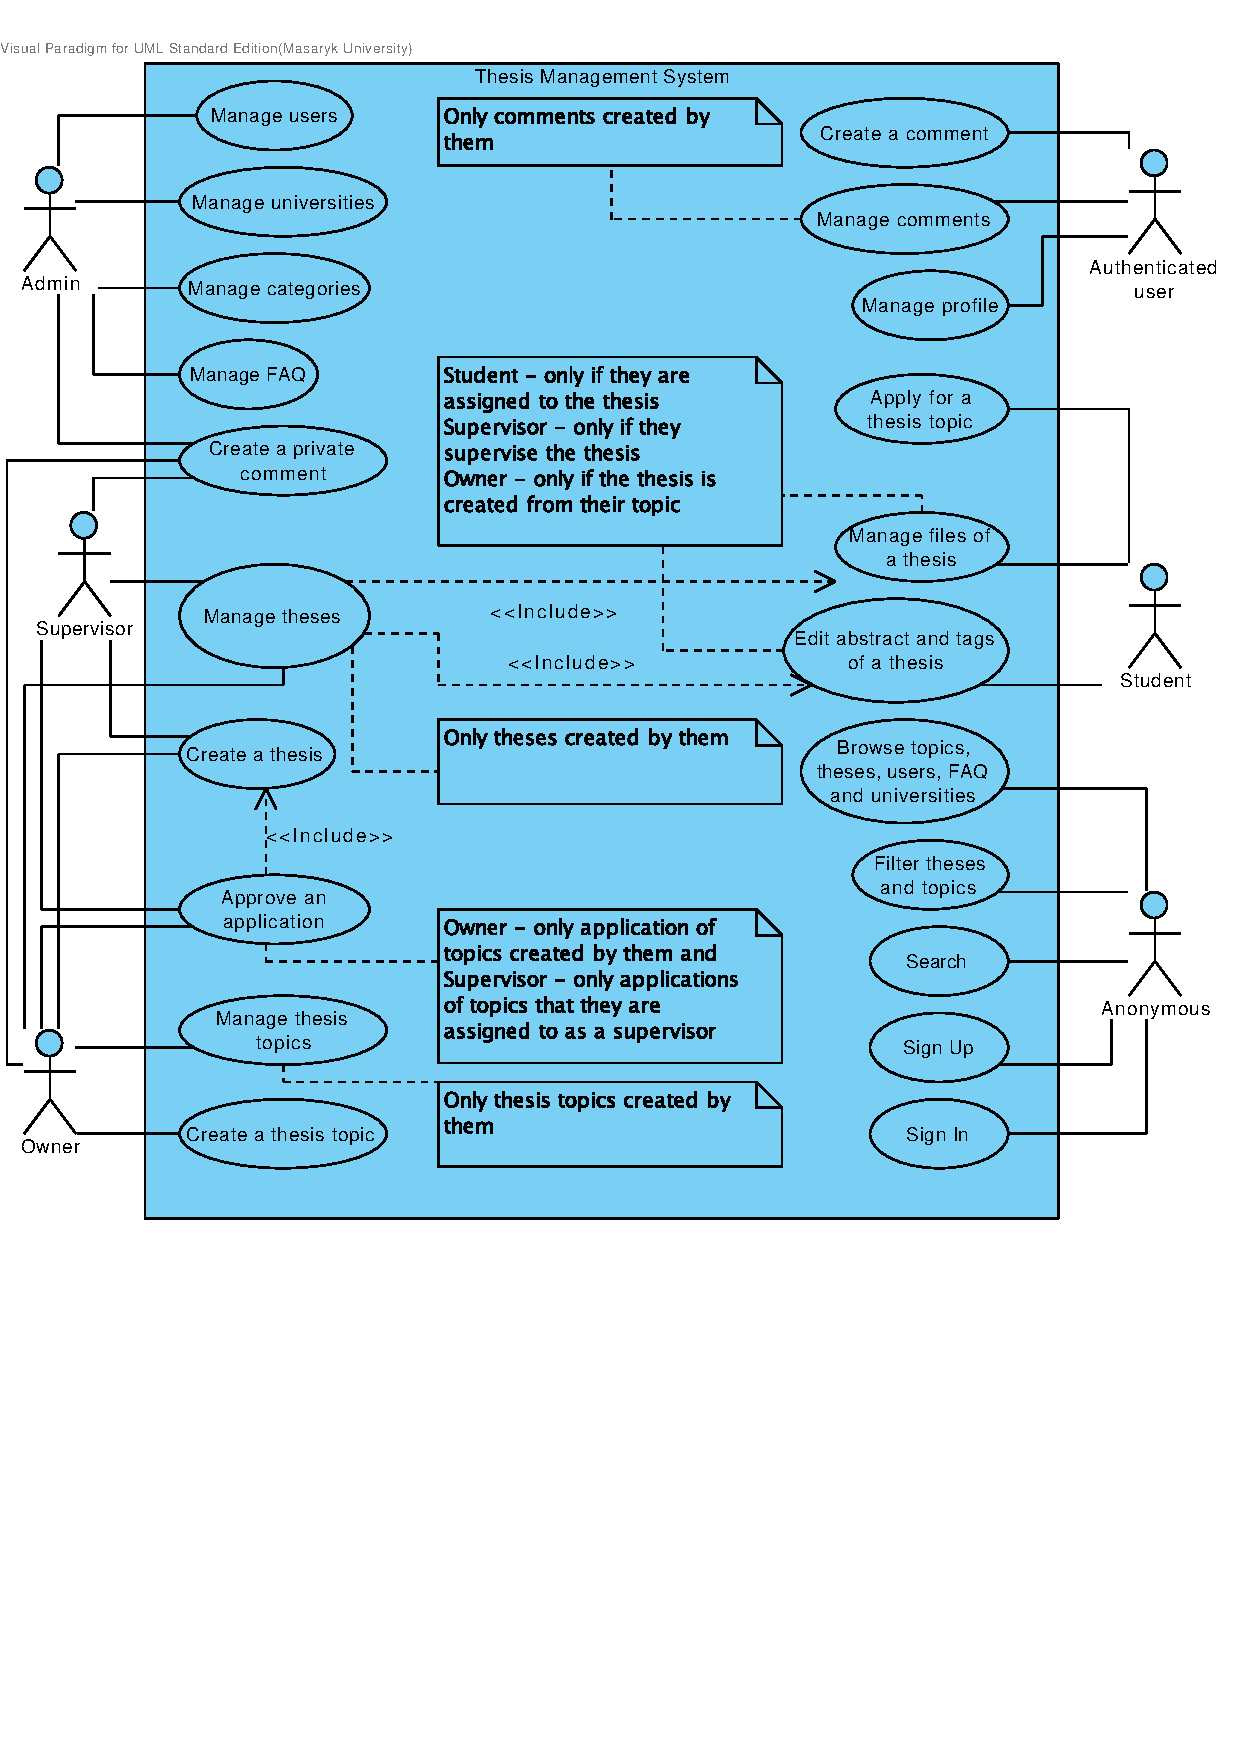
\includegraphics[trim=0 190 10 30, clip, keepaspectratio, width=\textwidth]{./images/use-case.pdf}
    \caption{Use case diagram of the Thesis Management System}
    \label{fig:use-case}
\end{figure}

\section{Non-Functional Requirements}

\begin{enumerate}
    \item Grails platform\\
    The system is implemented using platform Grails.

    \item Authentication and authorization\\
    The system is secured and there are four roles -- \textbf{Administrator} that can manage users, categories, FAQ and universities, \textbf{Leader} that can create thesis topics and manage thesis topics created by them, \textbf{Supervisor} that can create theses and manage theses created by them and \textbf{Student} that can apply for a thesis topic.

    \item Performance\\
    The system offers reasonable performance at least up to five hundred created thesis topics, theses, users and universities.

    \item Deployment\\
    The system is deployed on OpenShift using any cartridge other than Do It Yourself.

    \item License\\
    The system is licensed under any GPL compatible license.

    \item Backup\\
    Create a shell script for backing up the database.

    \item Internationalization and localization\\
    The system is internationalized and localized in English and Czech.

    \item Software development methodology\\
    The system is developed iteratively and incrementally.

\end{enumerate}

\section{Domain Model}

Designing the domain model is the most important step when designing an information system. It is also the most difficult one, because you usually cannot easily make changes in the domain model after you implemented the application logic around it. You can, however, add some domain model elements that the already-designed elements do not relate to. For example, if you design an entity \texttt{User}, you can implement it and easily add new entity \texttt{Group} later on if the \texttt{Group} is the owner of the relationship, see fig. \ref{fig:user-group-owner-example}. If the \texttt{User} is the owner of the relationship (see fig. \ref{fig:user-owner-group-example}), more refactoring is required to implement such changes (especially in case of object composition), because the fundamental API of the implemented part of the system changed.

\begin{figure}[h]
    \centering
        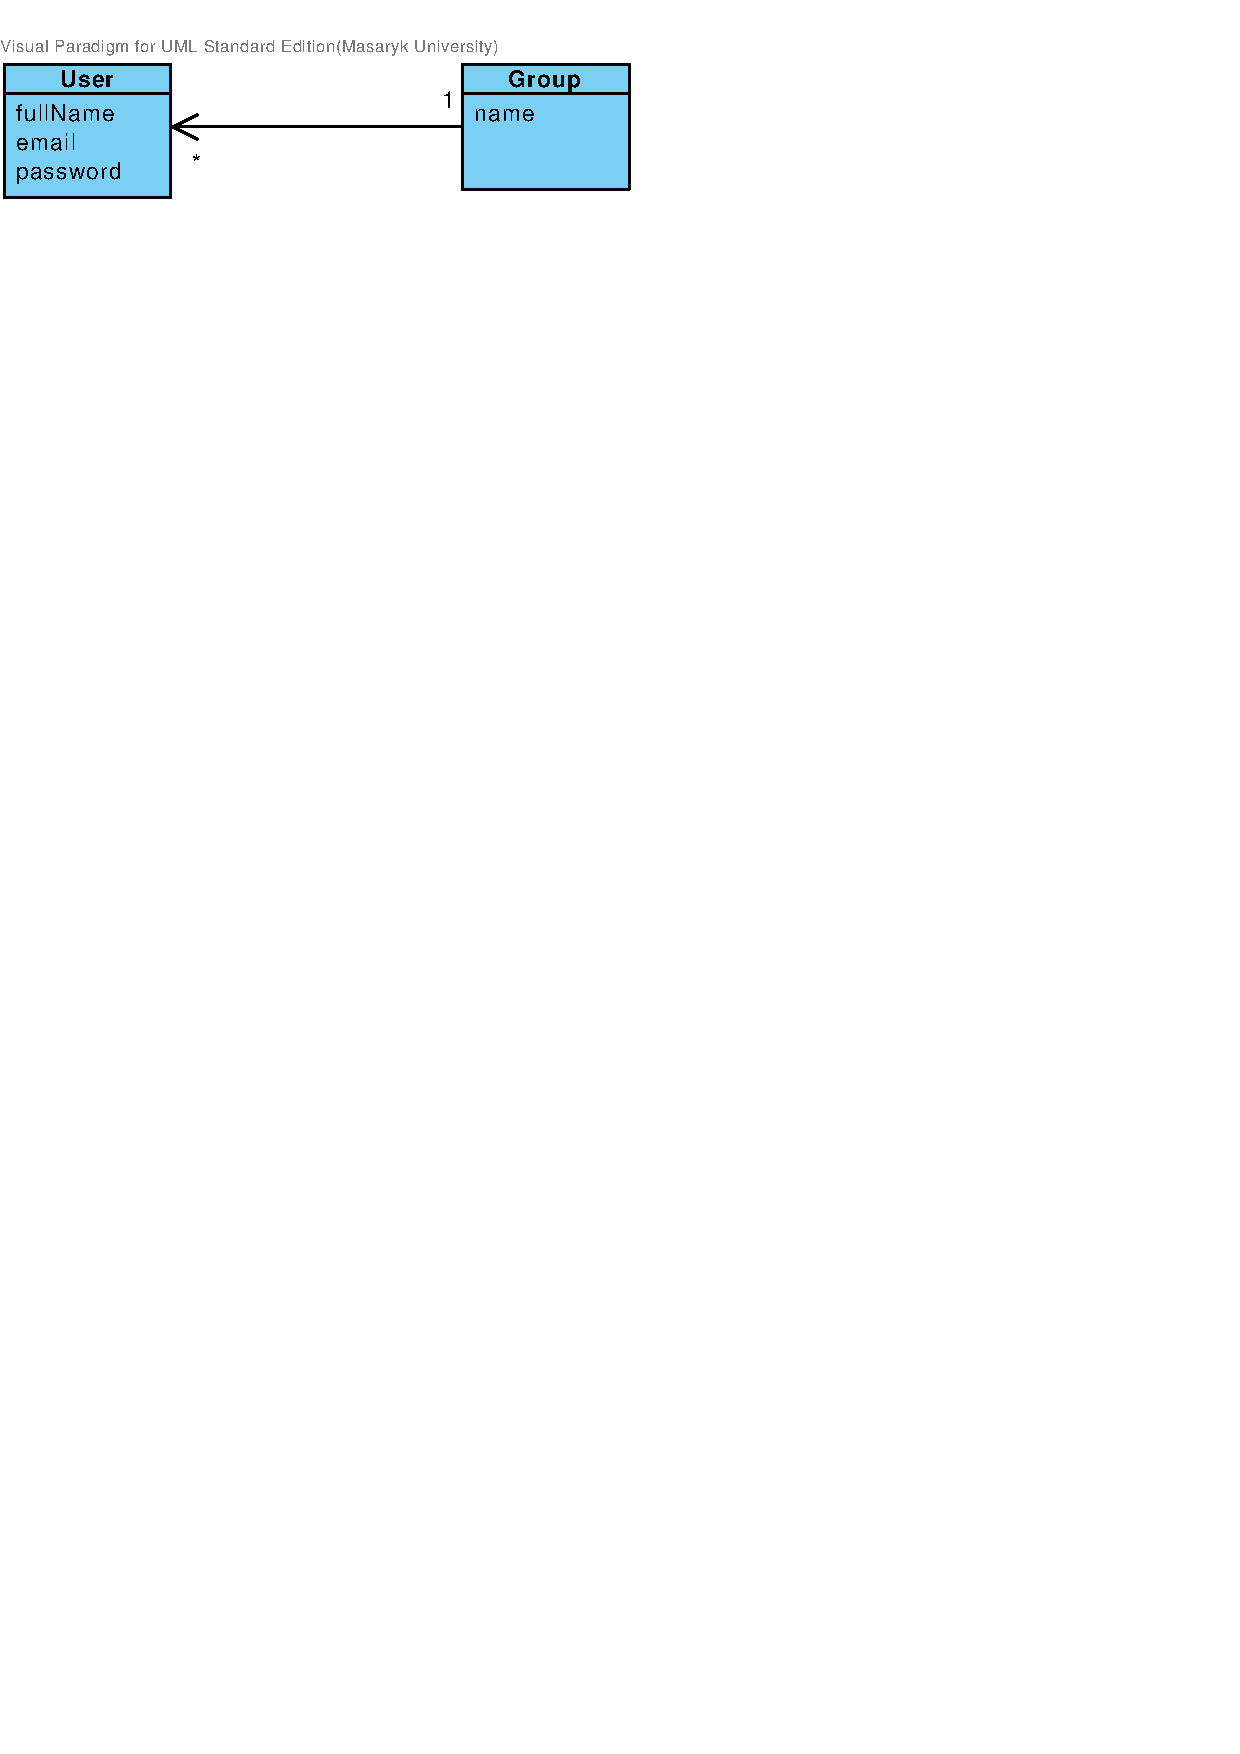
\includegraphics[trim=0 740 290 30, clip, keepaspectratio]{./images/user-group-owner-example.pdf}
    \caption{Example of domain model where \texttt{Group} owns the relationship}
    \label{fig:user-group-owner-example}
\end{figure}

\begin{figure}[h]
    \centering
        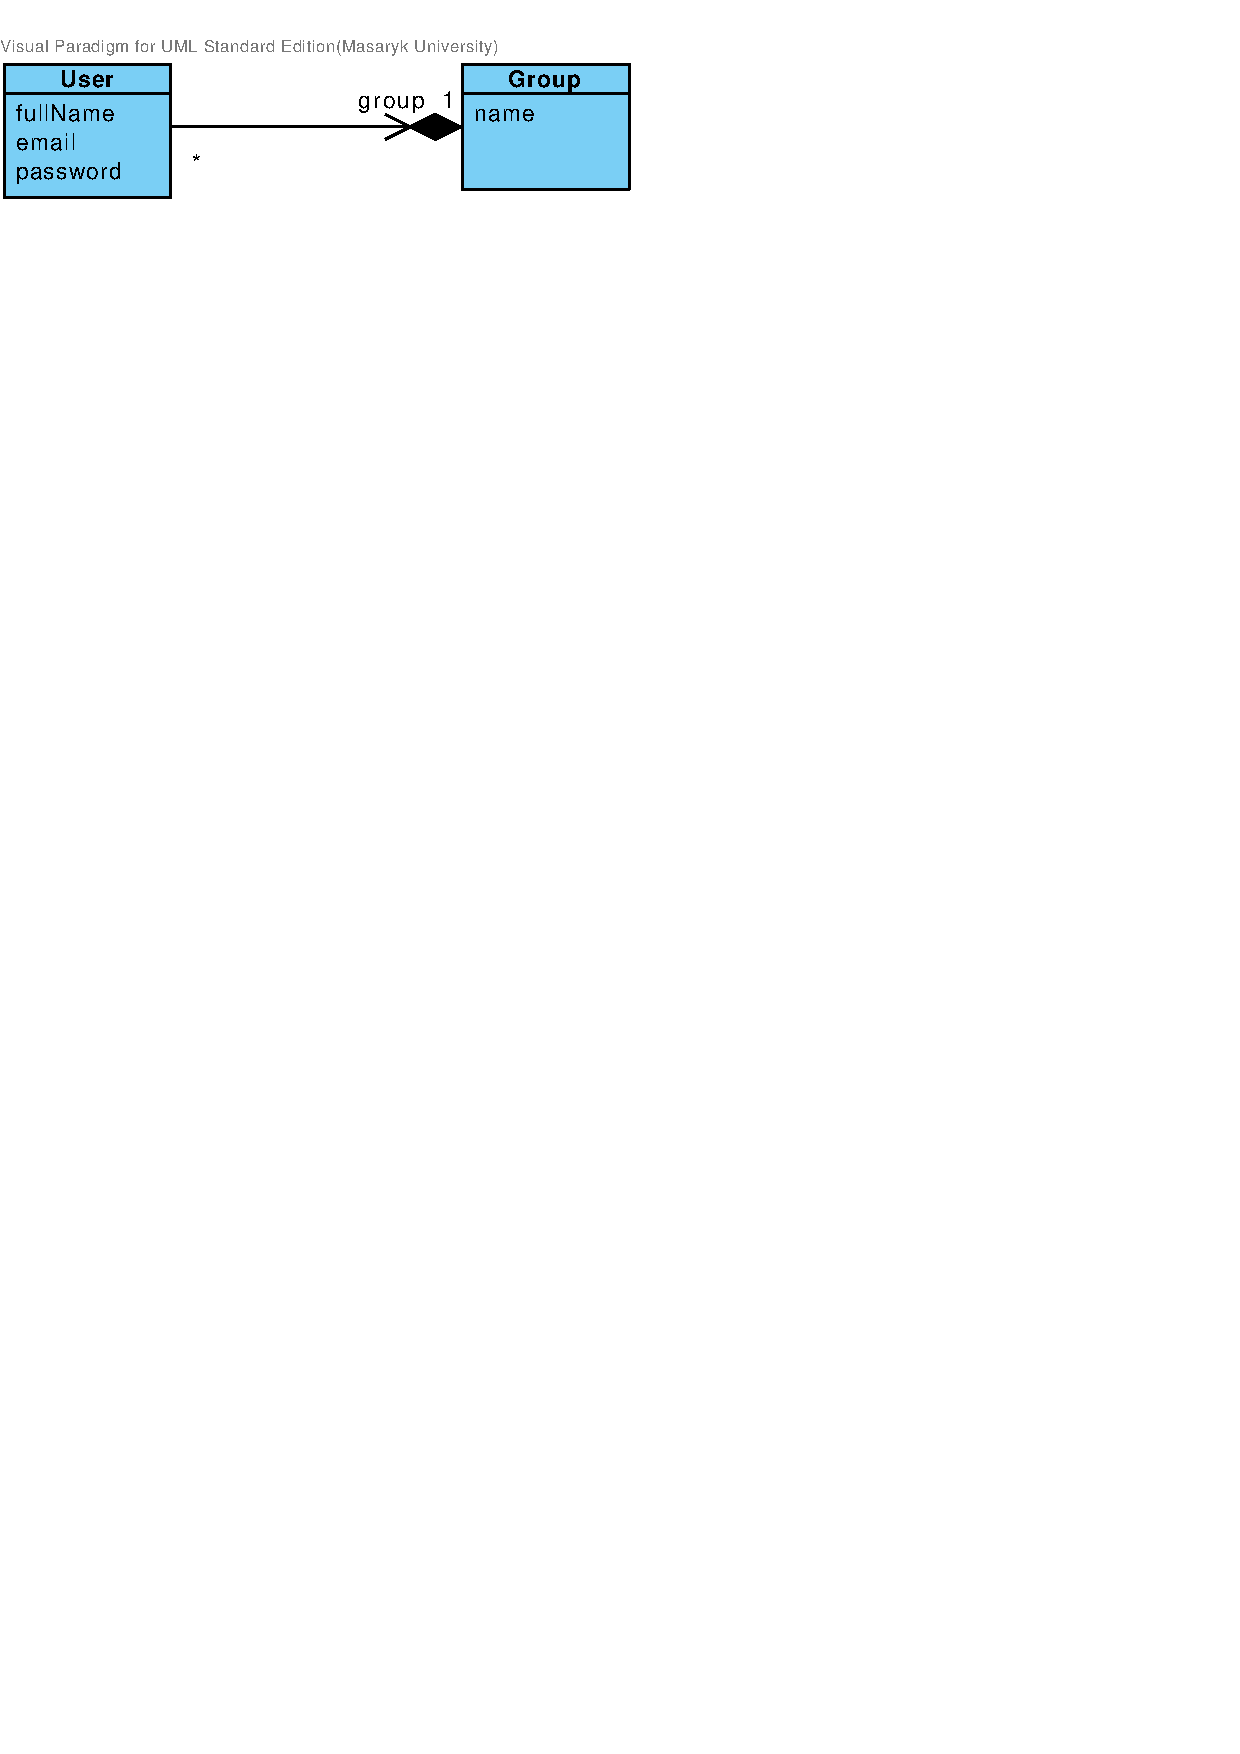
\includegraphics[trim=0 740 290 30, clip, keepaspectratio]{./images/user-owner-group-example.pdf}
    \caption{Example of domain model where \texttt{User} owns the relationship and composition is introduced}
    \label{fig:user-owner-group-example}
\end{figure}

Even more difficult can be deleting or editing attributes of an implemented entity. As a lot of refactoring is necessary to cope with such changes, a lot of new bugs is usually introduced, so it is best to avoid such changes by designing the domain model thoroughly.

Note that it is necessary to change the domain model if you implement your application incrementally. You should, however, try to minimize changes that require the API of the implemented domain model to be changed.

\subsection{Domain Model of the Thesis Management System}

As the domain model of the Thesis Management System is very complex, the author will describe it part by part. The complete domain model can be found in the appendix A.

\subsubsection{\texttt{User} entity}

To fulfill the first three functional requirements, we need to register users. For that reason, we introduce entity \texttt{User} with fields \texttt{email} and \texttt{password} that serve as log in credentials and field \texttt{fullName}. We also need fields \texttt{accountLocked} to allow the administrator to lock a user account and \texttt{enabled} for registration confirmation purposes. Field \texttt{sendMail} represents user setting that allows them to disable receiving notifications by email and field \texttt{dateCreated} represents the date of registration. To implement authorization, the \texttt{User} entity needs field \texttt{roles} which contains list of user's authorities. Figure \ref{fig:domain-user-entity} illustrates the described model.

\begin{figure}[h]
    \centering
        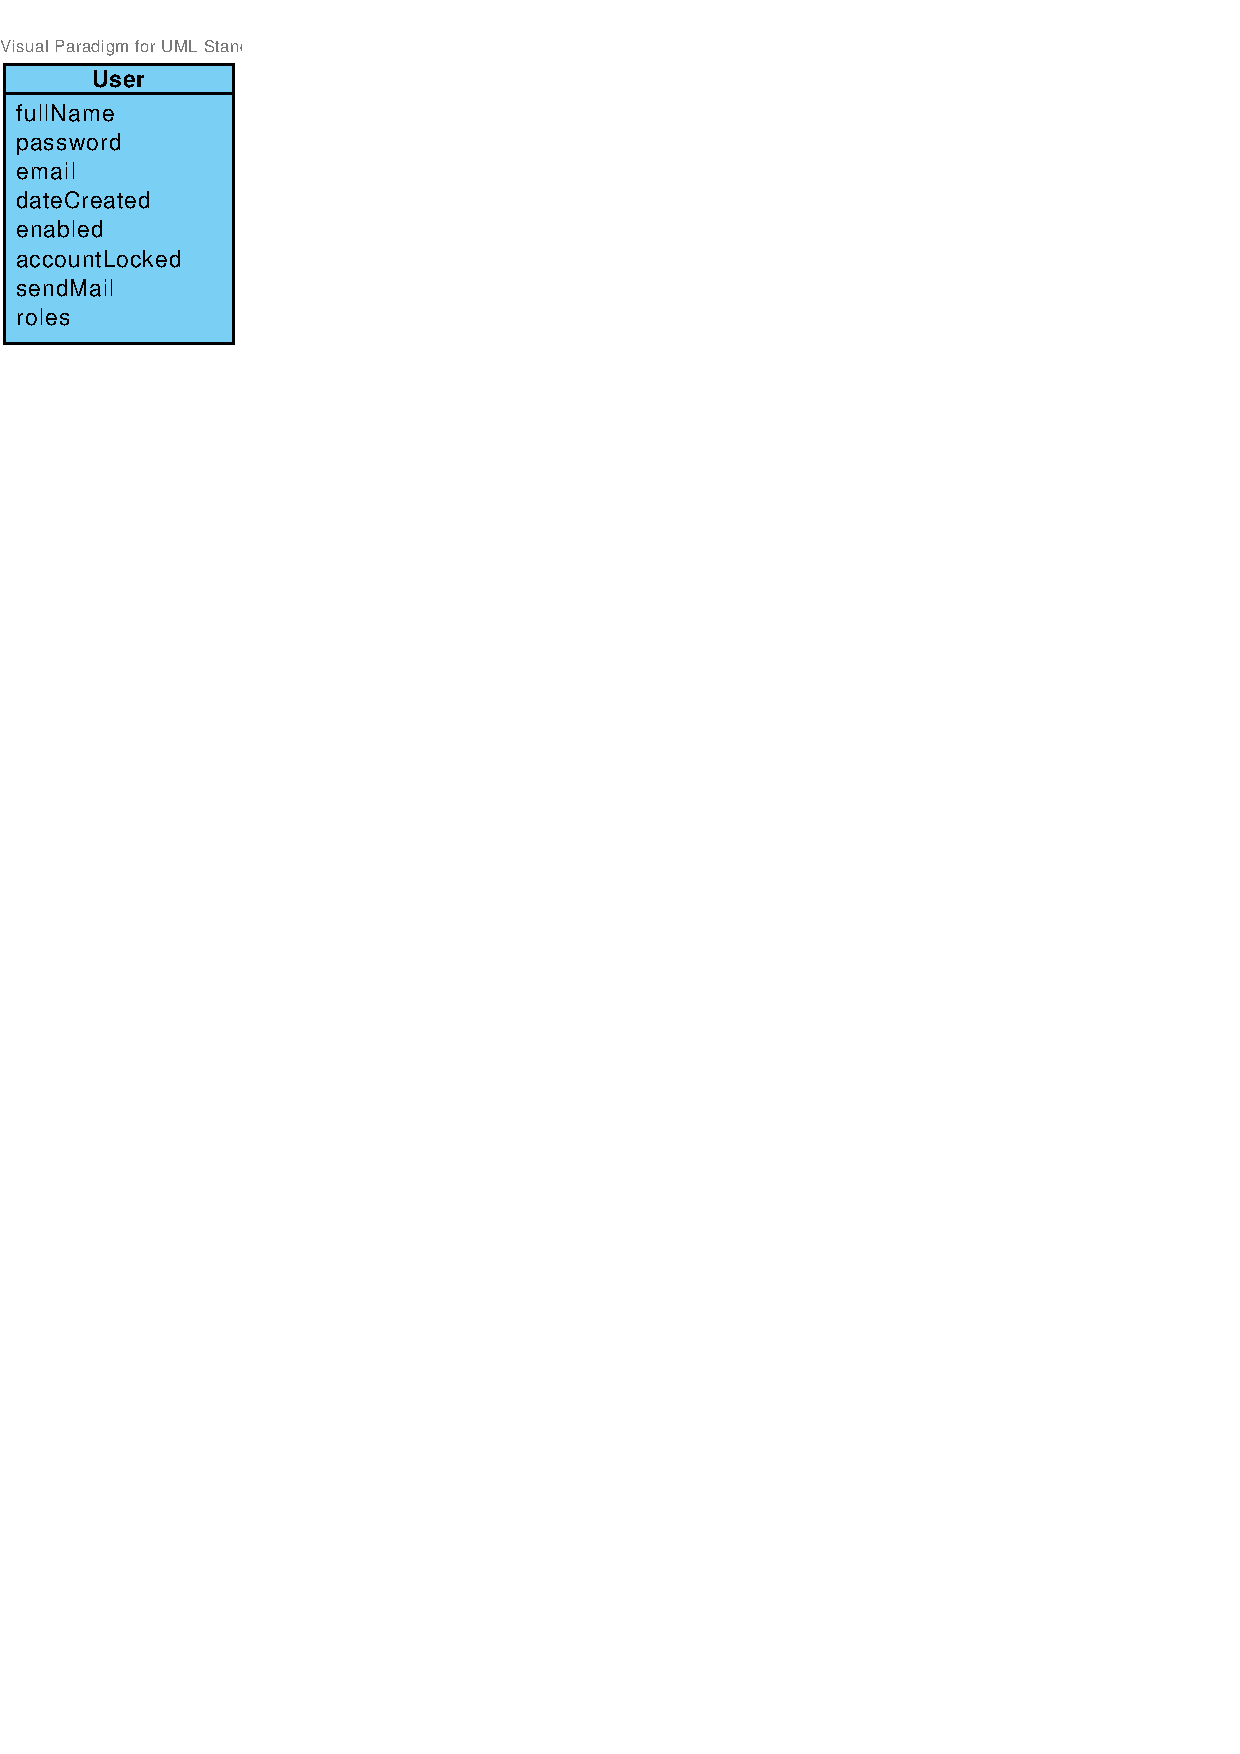
\includegraphics[trim=0 675 480 30, clip, keepaspectratio, scale=0.8]{./images/domain-user-entity.pdf}
    \caption{Model of \texttt{User} entity}
    \label{fig:domain-user-entity}
\end{figure}

\subsubsection{\texttt{University} entity}

To be able to keep a record of universities that a thesis topic is offered to, we need the entity \texttt{University} with only one field -- \texttt{name}, see Figure \ref{fig:domain-university-entity}.

\begin{figure}[h]
    \centering
        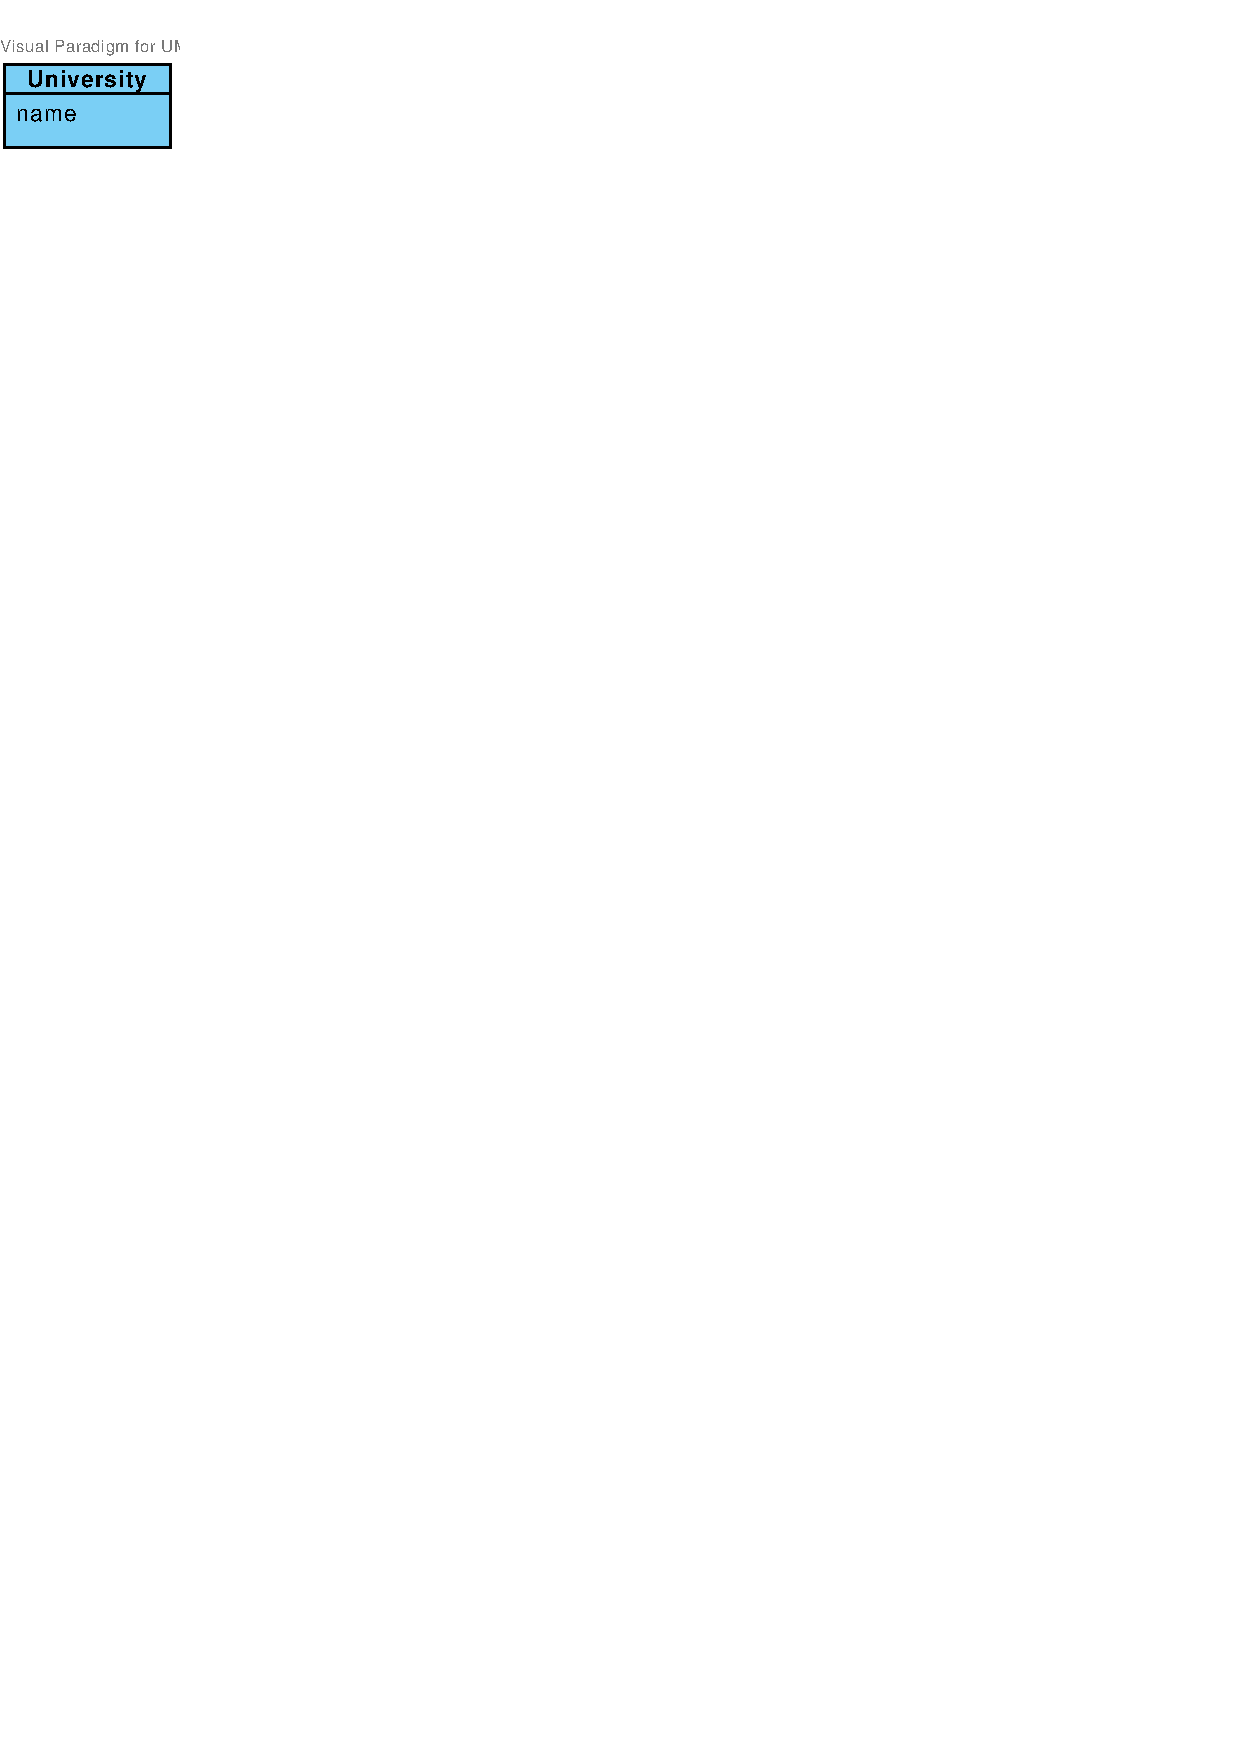
\includegraphics[trim=0 770 510 30, clip, keepaspectratio]{./images/domain-university-entity.pdf}
    \caption{Model of \texttt{University} entity}
    \label{fig:domain-university-entity}
\end{figure}

\subsubsection{\texttt{Article}, \texttt{Comment} and \texttt{Subscription} entities}

To allow users to add comments to thesis topics and theses, we need an entity that represents comments. The name of the entity is, for obvious reasons, \texttt{Comment} and fields that the entity requires are:

\begin{itemize}
    \item \texttt{content} -- represents the content of the comment
    \item \texttt{privateComment} -- mark if the comment is private
    \item \texttt{dateCreated} -- the date of creation, this field is used for sorting the comments so that we could show the user comments in either descending or ascending order
\end{itemize}

There are two association we need to create for \texttt{Comment}. First is a many-to-one association between \texttt{Comment} and \texttt{User} to be able to display the author of a comment. Second is a bit more complicated because there are two approaches to associate comments with thesis topics and theses. We could either create a many-to-one association between entities \texttt{Comment} and \texttt{Topic} and between entities \texttt{Comment} and \texttt{Thesis} or we could use generalization and move the many-to-one association up from \texttt{Thesis} and \texttt{Topic} to their parent. We choose the later approach because it allows us to create another ``commentable'' entity in the future simply by making it another child of the parent entity.

The \texttt{Article} entity represents the parent entity described above. We place the field \texttt{title} on it for reasons depicted in the following text.

The \texttt{Subscription} is only an association entity with no attributes on it but for the sake of future improvements, we model it separately. We could, for example, allow users to choose if they want to receive email notification for a particular subscription or let them set up what changes to an \texttt{Article} they want to be notified about. As far as associating the entity with other entities is concerned, it is very similar to the \texttt{Comment} entity because we need to implement subscription functionality for both topics and theses. We add the field \texttt{title} on the \texttt{Article} entity because we want to show subscribers the name of the \texttt{Article} that changed.

Described model is illustrated in Figure \ref{fig:domain-article-comment-subscription-entities}.

\begin{figure}[h]
    \centering
        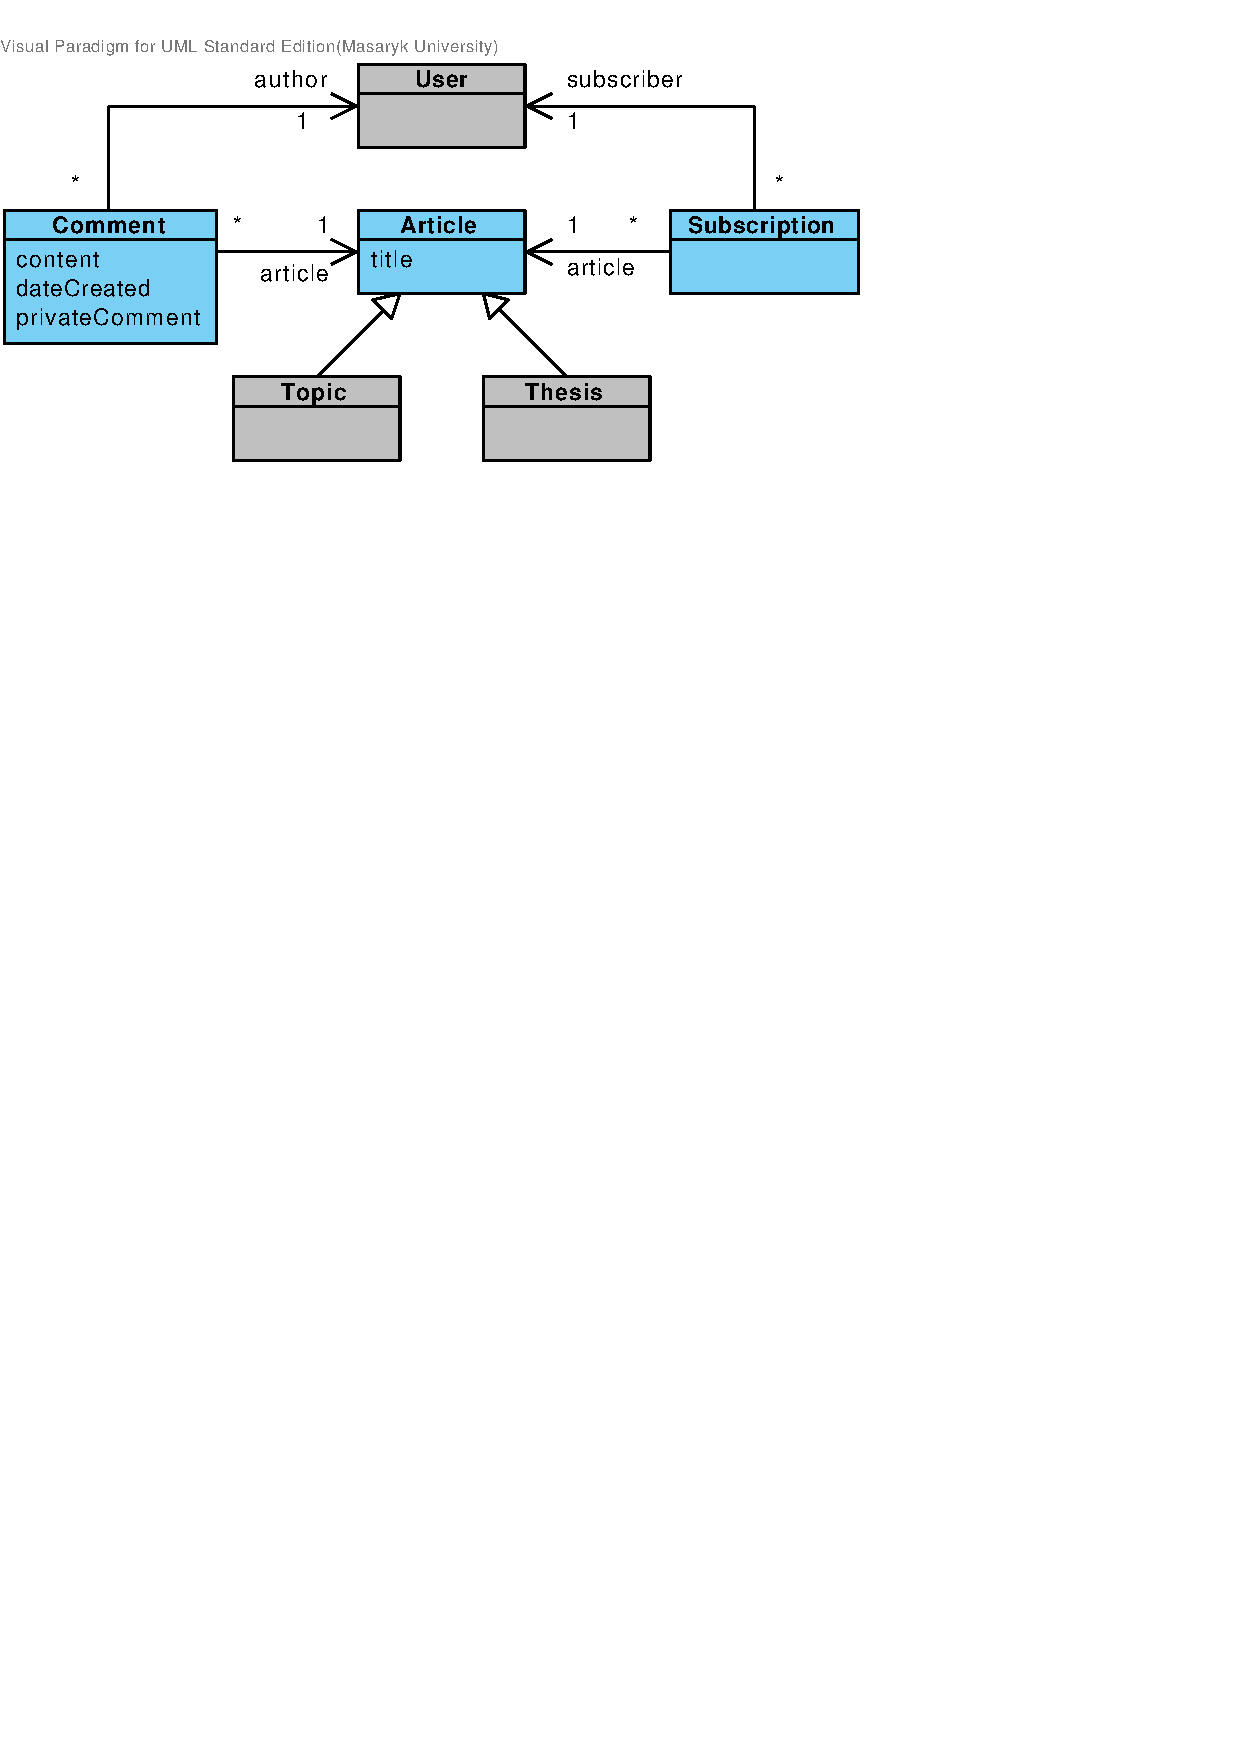
\includegraphics[trim=0 620 180 30, clip, keepaspectratio, width=\textwidth]{./images/domain-article-comment-subscription-entities.pdf}
    \caption{Model of \texttt{Article}, \texttt{Comment} and \texttt{Subscription} entities}
    \label{fig:domain-article-comment-subscription-entities}
\end{figure}

\subsubsection{\texttt{Feed} and \texttt{Notification} entities}

Entities \texttt{Feed} and \texttt{Notification} are quite closely related to the \texttt{Subscription} entity even though they are not directly associated. When a change is made to a topic or a thesis, the subscribers are notified by email and by a notification within the system. Emails are stored by the email hostings but the notifications need to be stored in the database of the Thesis Management System because they must be available to users when they visit the system.

Now, there are several ways how to implement such functionality but the most notable are the following two. The first approach is to create a \texttt{Notification} entity with fields including \texttt{message} that represents the content of the notification and associate it with the \texttt{User} entity that represents the subscriber. This approach is favorable because it is simple, however, it creates unnecessary redundancy in the database as a new notification with the same \texttt{message} is created for every subscriber. The second approach, which is used in the Thesis Management System, is to create another entity \texttt{Feed} and move the \texttt{message} field onto it. The later approach is also more suitable if we want to show the user a notification according to their locale setting. 

Figure \ref{fig:domain-feed-notification-entities} illustrates the model of this part of the system. Since we want the notifications to be localized, the \texttt{Feed} entity has fields \texttt{messageCode}, which represents the code of the massage to be displayed as a notification, \texttt{args}, which represents the arguments of the message and \texttt{dateCreated}, which allows us to sort the notifications to show users the latest notifications first. The \texttt{Feed} entity is also associated with the \texttt{User} entity which represents the user who triggered the creation of the feed. This allows us to find user's activity.

The \texttt{Notification} entity is basically an association entity between entities \texttt{User} and \texttt{Feed}. The field \texttt{seen} represents status of a notification, i.e. if the user has already seen the notification or not.

\begin{figure}[h]
    \centering
        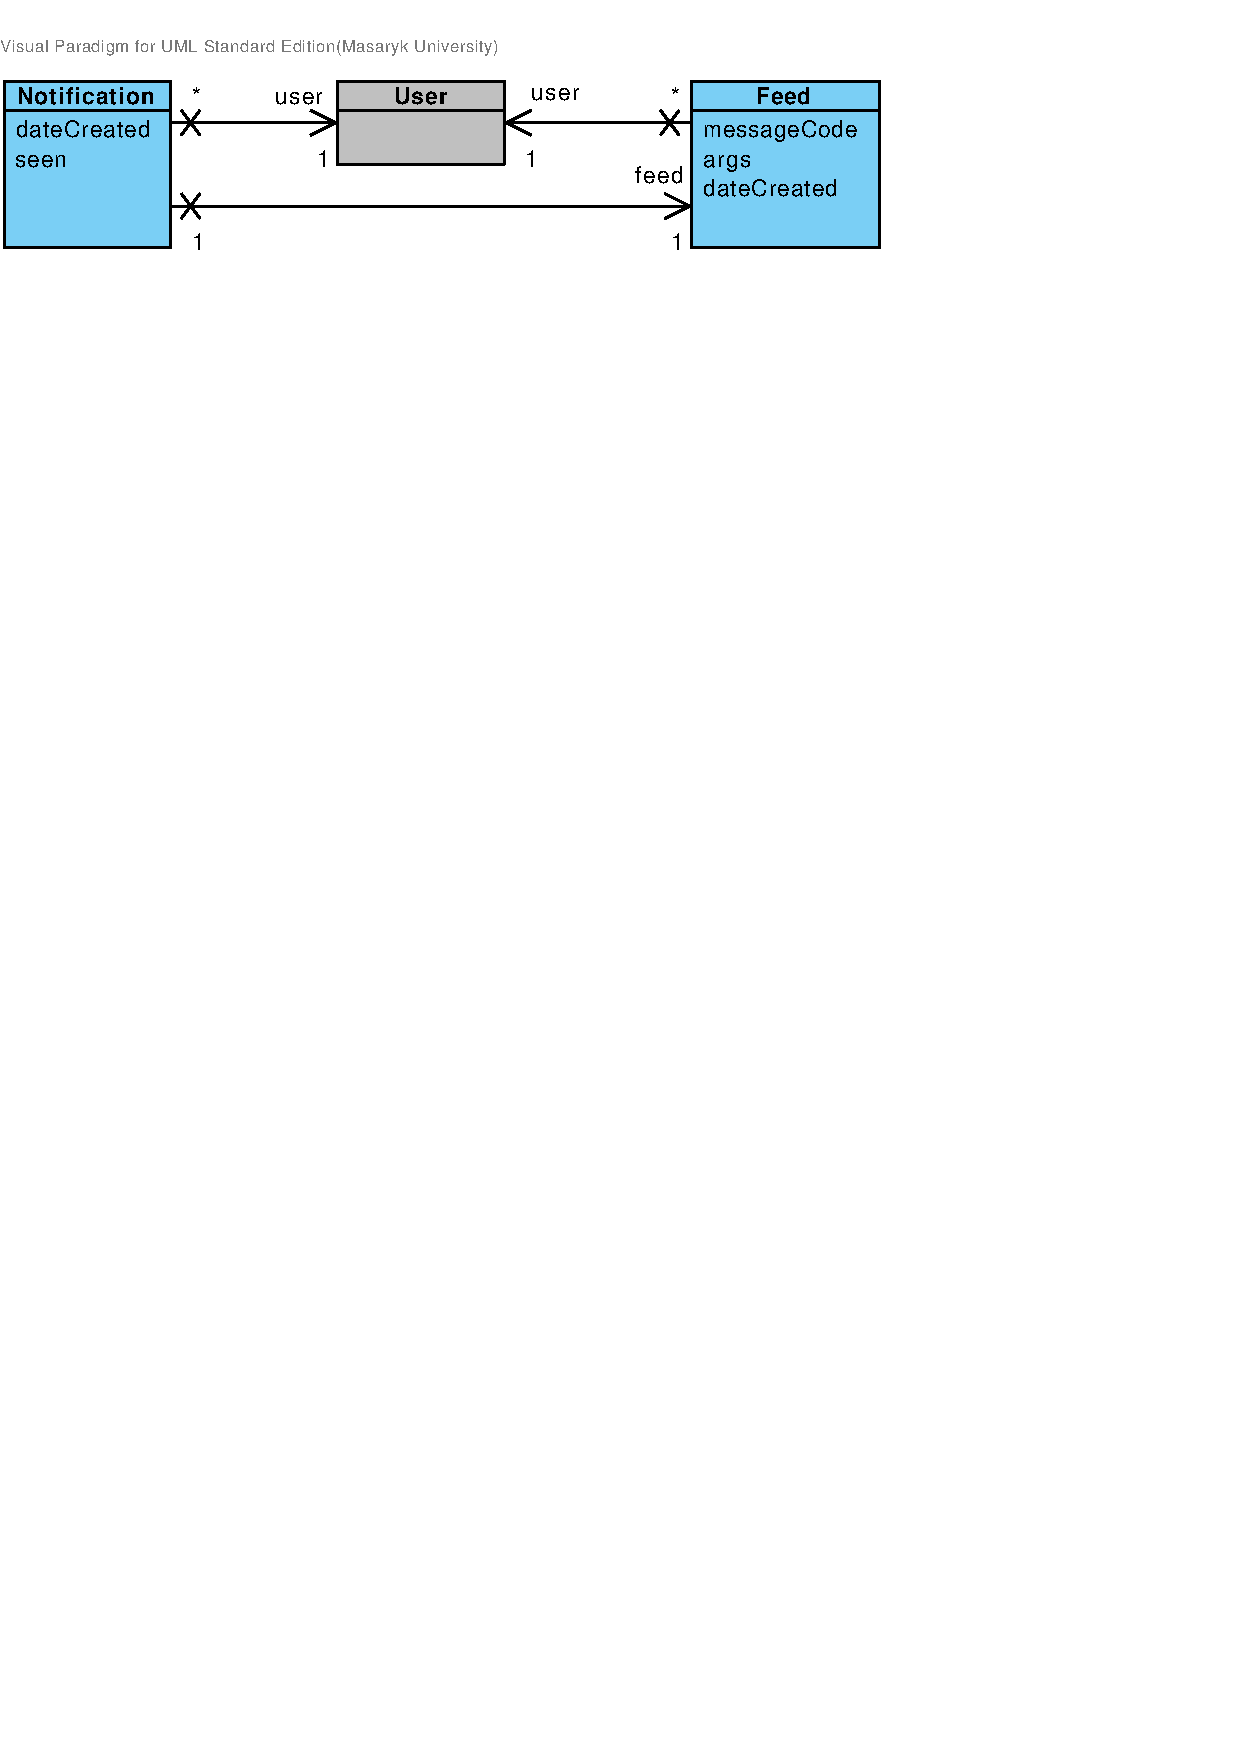
\includegraphics[trim=0 720 170 30, clip, keepaspectratio, width=\textwidth]{./images/domain-feed-notification-entities.pdf}
    \caption{Model of \texttt{Feed} and \texttt{Notification} entities}
    \label{fig:domain-feed-notification-entities}
\end{figure}

\subsubsection{\texttt{Tag} entity}

The most common way of implementing tags in an information system is to place collection of simple strings in an entity. We chose a different approach for the Thesis Management System, though. We introduced a separate entity \texttt{Tag} that contains a simple field \texttt{title}. Making the \texttt{Tag} entity separate makes it easy to add new fields on it in the future, e.g. \texttt{description}, and it is easier to aggregate, for example, number of all tags used in the system. Figure \ref{fig:domain-tag-entity} depicts the model.

\begin{figure}[h]
    \centering
        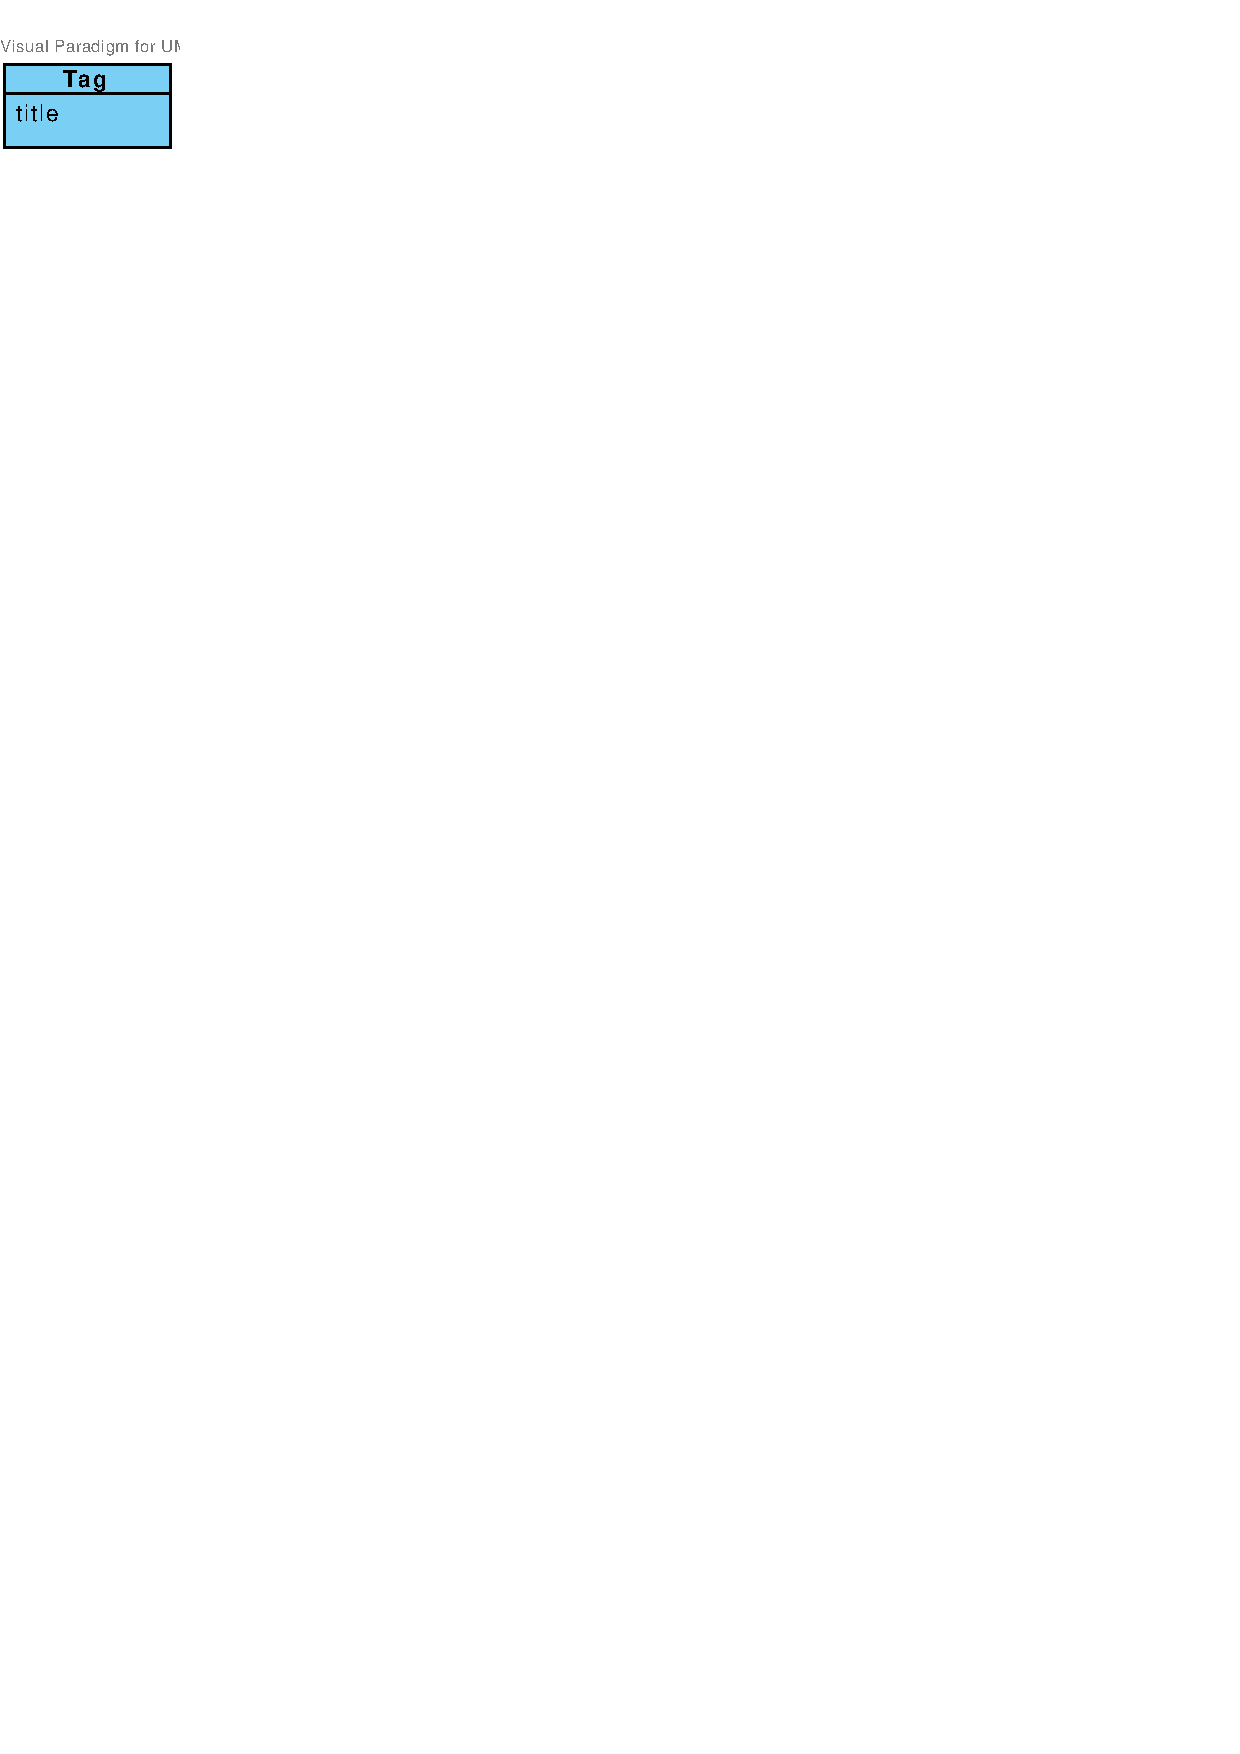
\includegraphics[trim=0 770 510 30, clip, keepaspectratio]{./images/domain-tag-entity.pdf}
    \caption{Model of \texttt{Tag} entity}
    \label{fig:domain-tag-entity}
\end{figure}

\subsubsection{\texttt{Topic}, \texttt{Category} and \texttt{Supervision} entitites}

\texttt{Topic} is the most important entity in the system because it represents the topic of a thesis. It is a child entity of the \texttt{Article} entity which means that the \texttt{title} field is included in the \texttt{Topic} entity automatically. Description of the other fields follows:

\begin{itemize}
    \item \texttt{secondaryTitle} -- Represents the title of the topic in a different language (e.g. Czech, Slovak).
    \item \texttt{lead} -- Lead paragraph, is displayed on the page with the list of topics.
    \item \texttt{Description} -- Description of the topic.
    \item \texttt{secondaryDescription} -- Represents the description of the topic in a different language.
    \item \texttt{dateCreated} -- The date of creation of the topic.
    \item \texttt{enabled} -- Flag which marks a topic that is enabled or disabled, i.e. students can(not) apply for it.
    \item \texttt{types} -- Collection of types of the topic (e.g. bachelor, diploma).
\end{itemize}

The \texttt{Topic} entity also has a many-to-many association with the \texttt{Tag} entity and the \texttt{User} entity which represents the leader of the topic, i.e. the user which created the topic and is in charge of it. The association with the \texttt{University} entity is necessary to keep a record of universities that the topic is offered to, i.e. students of what universities can apply for it.

Another requirement of the system is to place topics in categories. Categories are represented by the \texttt{Category} entity which has only two fields -- the \texttt{name} field which represents the name of the category and the \texttt{description} field which is self-explanatory. The \texttt{Topic} entity is associated with the \texttt{Category} entity in a many-to-many manner. In the first stages of the design, we expected the categories to be hierarchical, i.e. a category could have several subcategories, but we decided to abolish such approach as it would place unnecessary overhead on the database.

The most difficult part of the system was to design the requirement allowing topics to list university supervisors. There are zero or more supervisors in one topic but one supervisor can supervise a topic at multiple universities which means that the supervisors cannot be associated with the \texttt{Topic} entity directly. Instead, we introduced the \texttt{Supervision} entity which is basically an association entity without any fields representing a supervisor associated with a university.

Described design is depicted in Figure \ref{fig:domain-topic-category-supervision-entities}.

\begin{figure}[h]
    \centering
        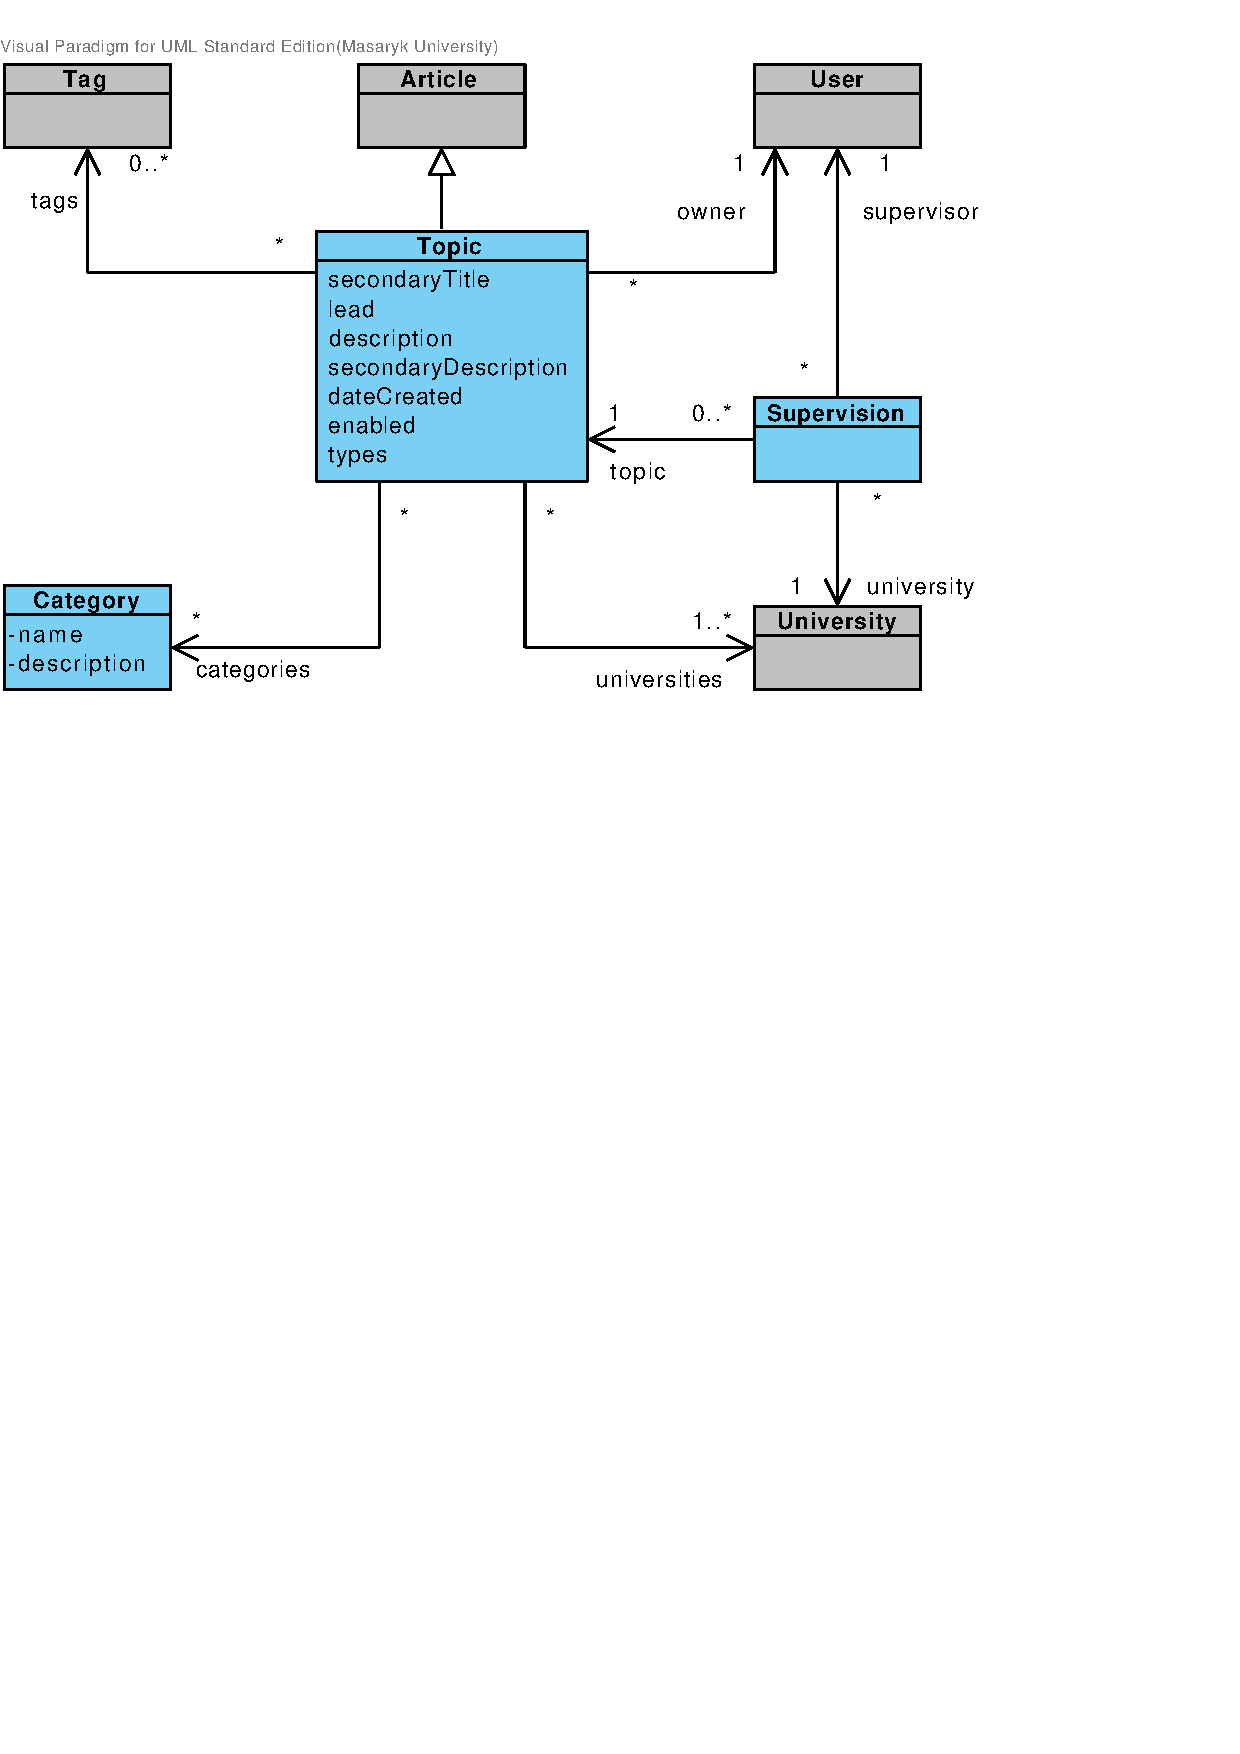
\includegraphics[trim=0 510 120 30, clip, keepaspectratio, width=\textwidth]{./images/domain-topic-category-supervision-entities.pdf}
    \caption{Model of \texttt{Topic}, \texttt{Category} and \texttt{Supervision} entities}
    \label{fig:domain-topic-category-supervision-entities}
\end{figure}

\subsubsection{\texttt{Thesis} entity}

The second most important entity of the system is the \texttt{Thesis} entity, it represents an academic project of a student and it is associated with the \texttt{Topic} entity. There can be multiple theses created from one topic for several reasons:

\begin{itemize}
    \item One topic can be intended for several students (for example when the topic is too difficult for one student) which means that a thesis for each student needs to be created.
    \item The topic is offered in more than one semester.
    \item The student that was assigned to the thesis of a topic failed to finish with a satisfactory result and the topic has to be offered again.
\end{itemize}

This means that the cardinality of the association with the \texttt{Topic} entity must be a many-to-one one.

The \texttt{Thesis} entity is, as well as the \texttt{Topic} entity, a child of the \texttt{Article} entity which takes care of the title, comments and subscriptions. Theses are not required to be stored in two languages which means that there is no need for both the secondary title and the secondary description. There are several other fields required, though:

\begin{itemize}
    \item \texttt{description} -- Represents the official description of the thesis.
    \item \texttt{status} -- Status of the thesis which can be either `in progress', `finished', `failed' or `postponed'.
    \item \texttt{grade} -- If the thesis is finished, a grade must be awarded. The grade can be one of the following: A, B, C, D, E, F.
    \item \texttt{abstract} -- The abstract of the thesis provided by the assigned student.
    \item \texttt{dateCreated} -- The date of creation of the thesis.
    \item \texttt{type} -- The type of the thesis which can be for example `bachelor' or `diploma'.
    \item \texttt{notes} -- A field for the supervisor where they can leave notes related to the thesis.
\end{itemize}

The student that is assigned to a thesis and the supervisor are represented by the associations with the \texttt{User} entity and the thesis university is represented by the one with the \texttt{University} entity. The tags of a thesis are designed the same way as with the \texttt{Topic} entity. The reason why the association with the \texttt{Tag} entity is not moved up to the \texttt{Article} entity is because in the future, there might be added a functionality for management of school projects that does not require tags but requires the functionality provided by the \texttt{Article} entity.

Figure \ref{fig:domain-thesis-entity} illustrates this model.

\begin{figure}[h]
    \centering
        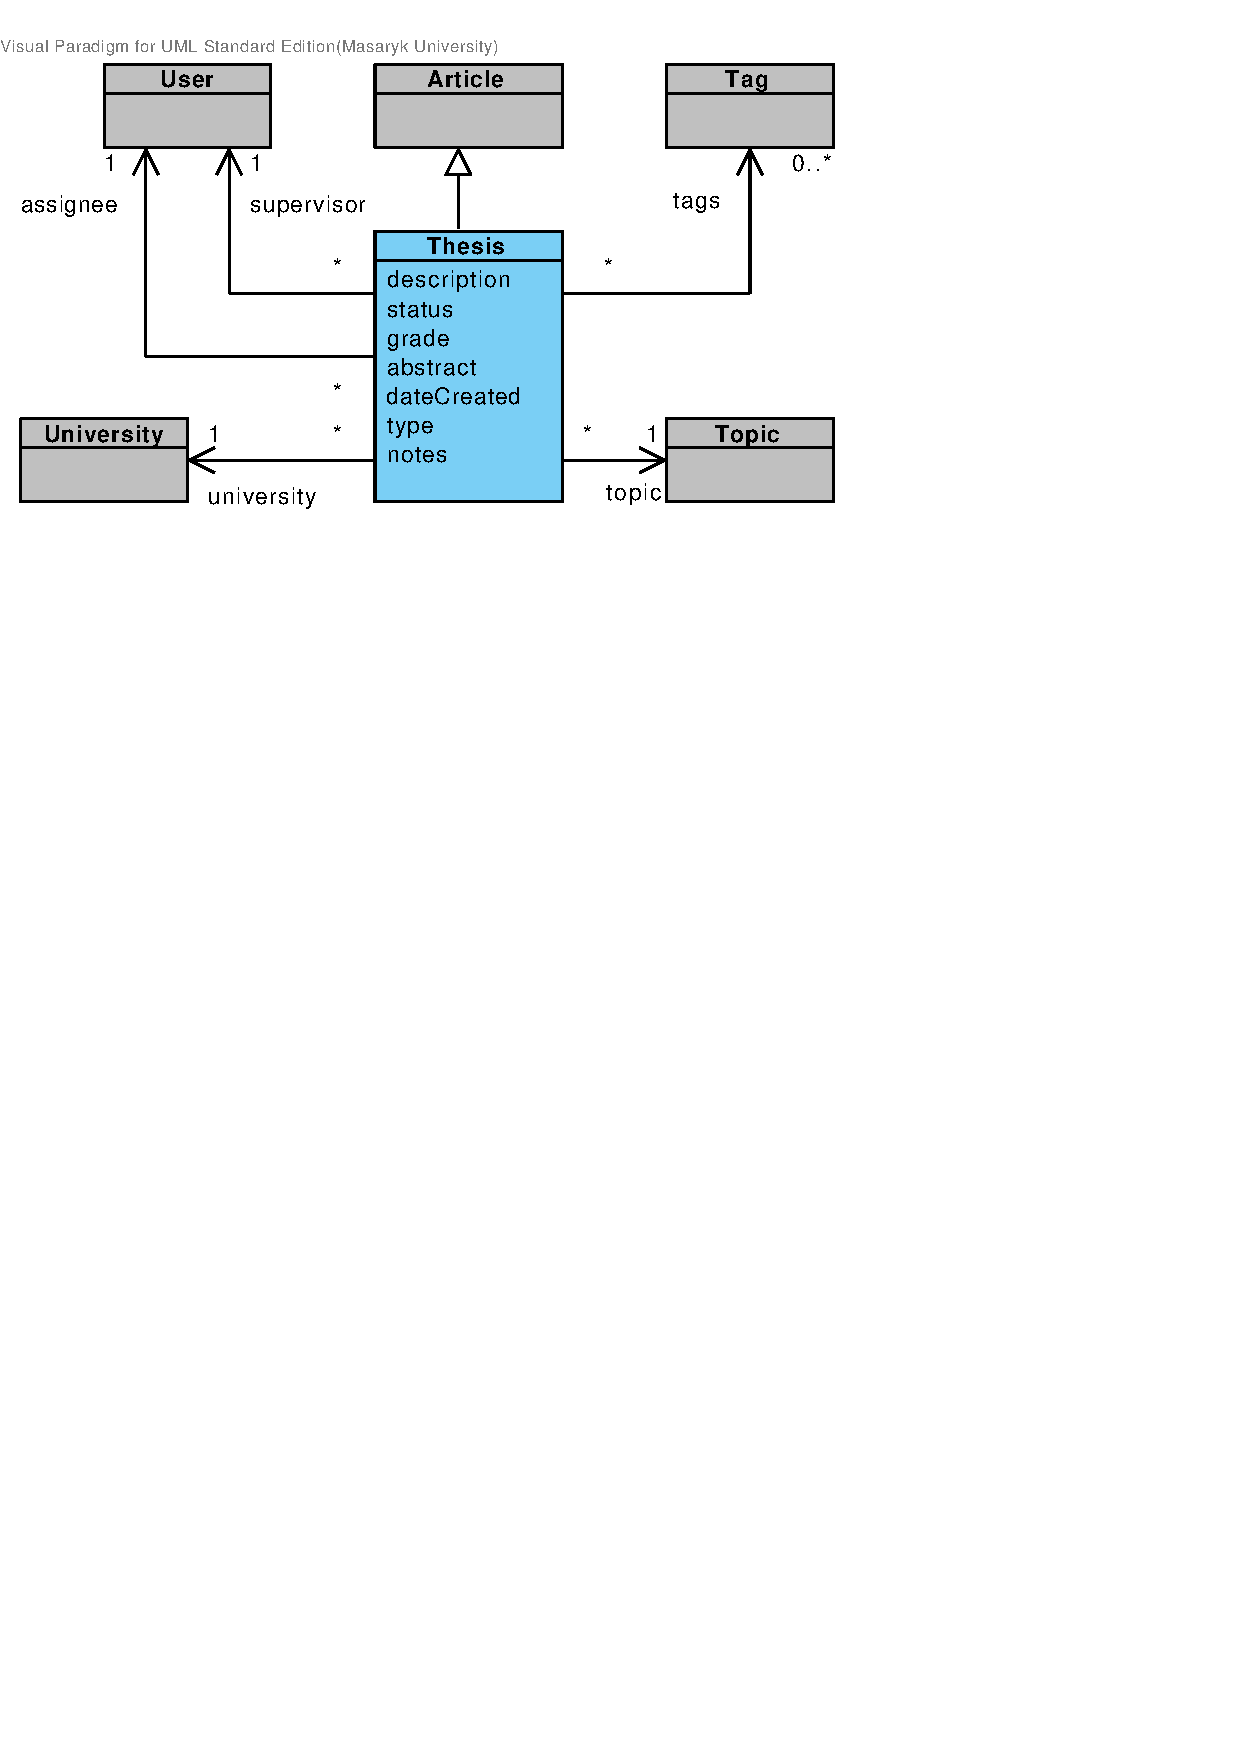
\includegraphics[trim=0 600 190 30, clip, keepaspectratio, width=\textwidth]{./images/domain-thesis-entity.pdf}
    \caption{Model of \texttt{Thesis} entity}
    \label{fig:domain-thesis-entity}
\end{figure}

\subsubsection{\texttt{Application} entity}

When a student applies for a topic, an application must be created to allow the leader or a supervisor of the topic to review and possibly approve it. To apply for a topic, a student must choose the type and the university for which they apply. The type is stored in the \texttt{type} field and the university is represented by the association with the \texttt{University} entity. The student can also leave a note, e.g. the preferred supervisor, which is stored in the \texttt{note} field. The \texttt{dateCreated} field allows the authority (leader or supervisor) to see which application was created first and the \texttt{approved} field marks applications that are already approved. The association with the \texttt{User} resp. \texttt{Topic} entity represents the student who applied for the topic resp. the topic that the application is created for. The association with the \texttt{Thesis} entity allows us to display the thesis that was created from an application. Note that this association has 0..1 multiplicity (in both directions). This is because when a student applies for a topic, the thesis is not created yet. The multiplicity from the other direction results from the fact that a thesis can be created directly from a topic (i.e. no application is created). This model is depicted in Figure \ref{fig:domain-application-entity}.

\begin{figure}[h]
    \centering
        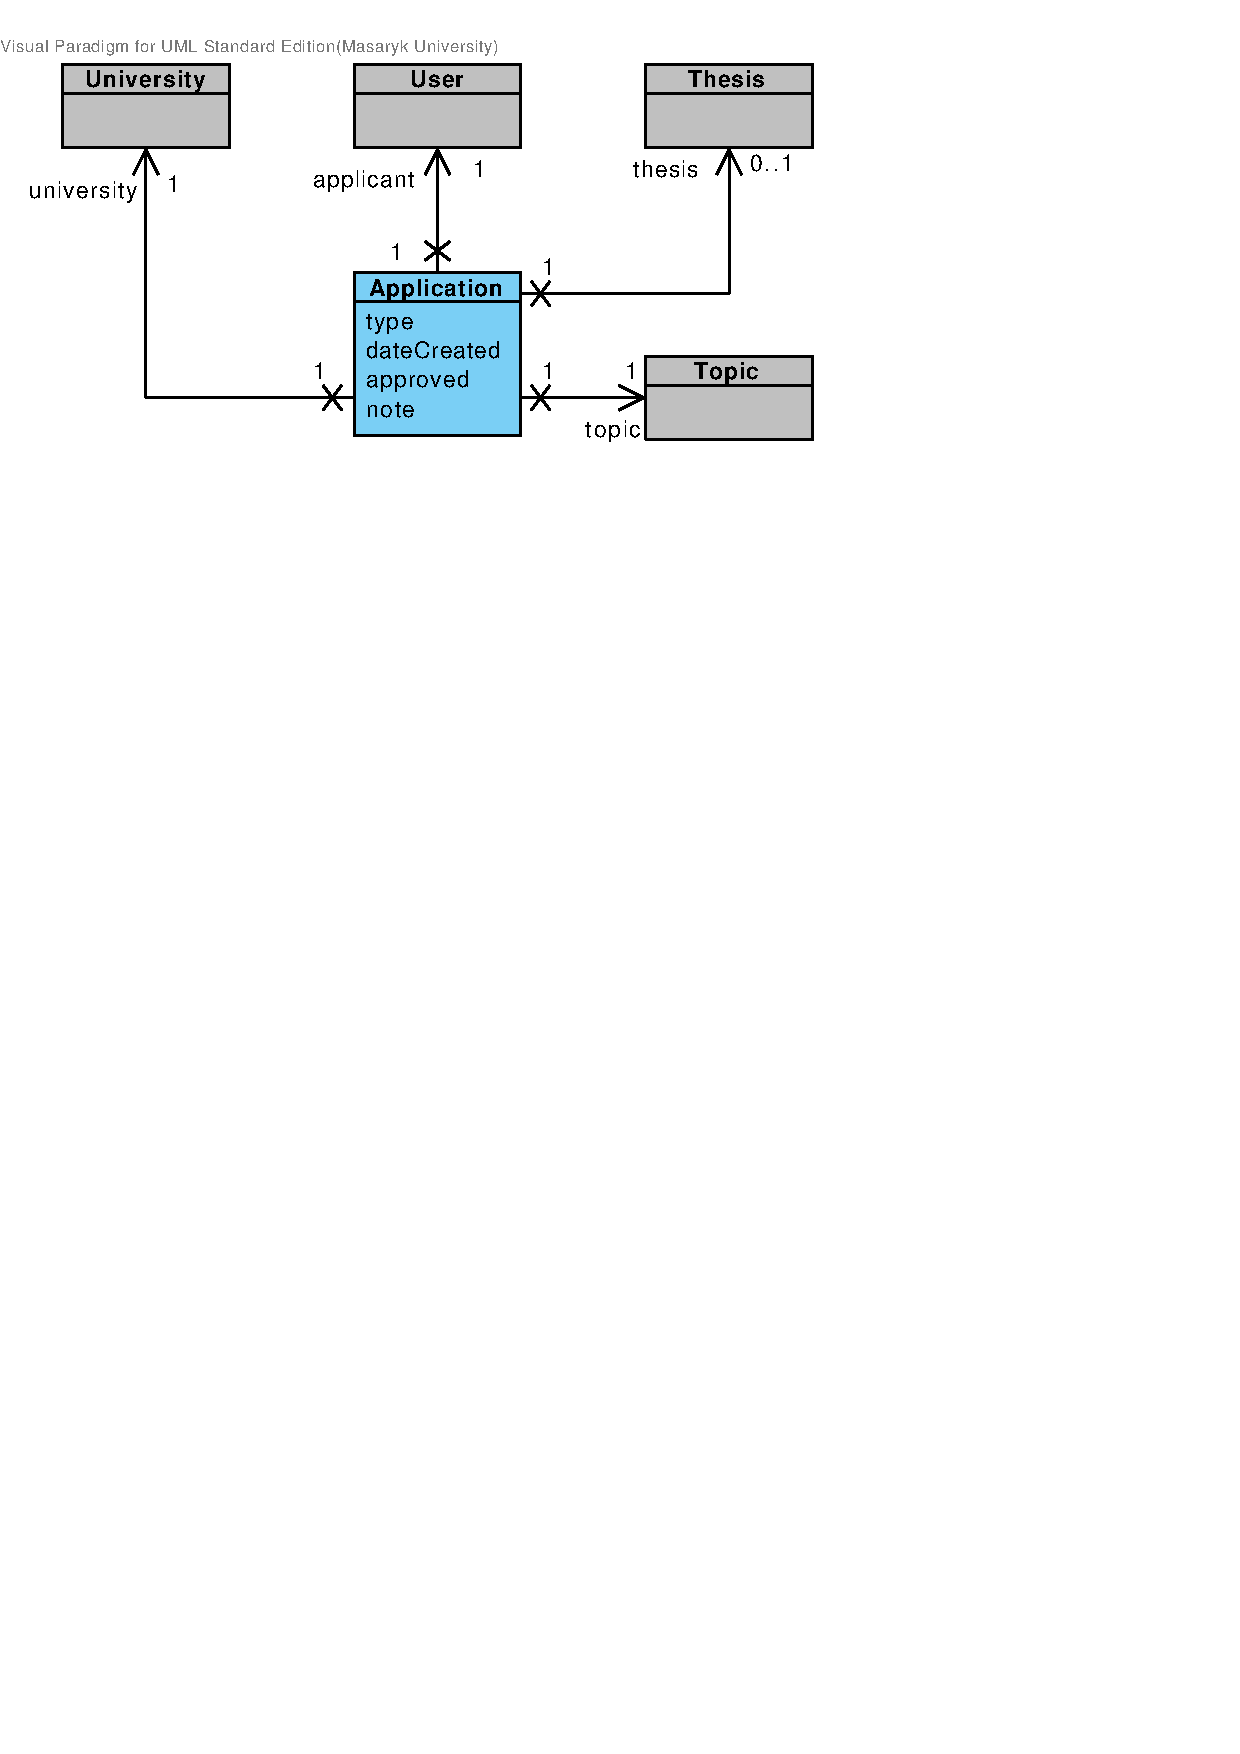
\includegraphics[trim=10 630 200 30, clip, keepaspectratio, width=\textwidth]{./images/domain-application-entity.pdf}
    \caption{Model of \texttt{Application} entity}
    \label{fig:domain-application-entity}
\end{figure}

\subsubsection{\texttt{Faq} entity}

To allow new users to adapt to a new system more quickly, Frequently Asked Questions are introduced. The FAQ are represented by the \texttt{Faq} entity with the following fields:

\begin{itemize}
    \item \texttt{question} -- The question to be answered.
    \item \texttt{answer} -- The answer to the frequently asked question.
    \item \texttt{locale} -- The locale of the group of users for which the frequently asked question is displayed.
\end{itemize}

See figure \ref{fig:domain-faq-entity} to see the designed model.

\begin{figure}[h]
    \centering
        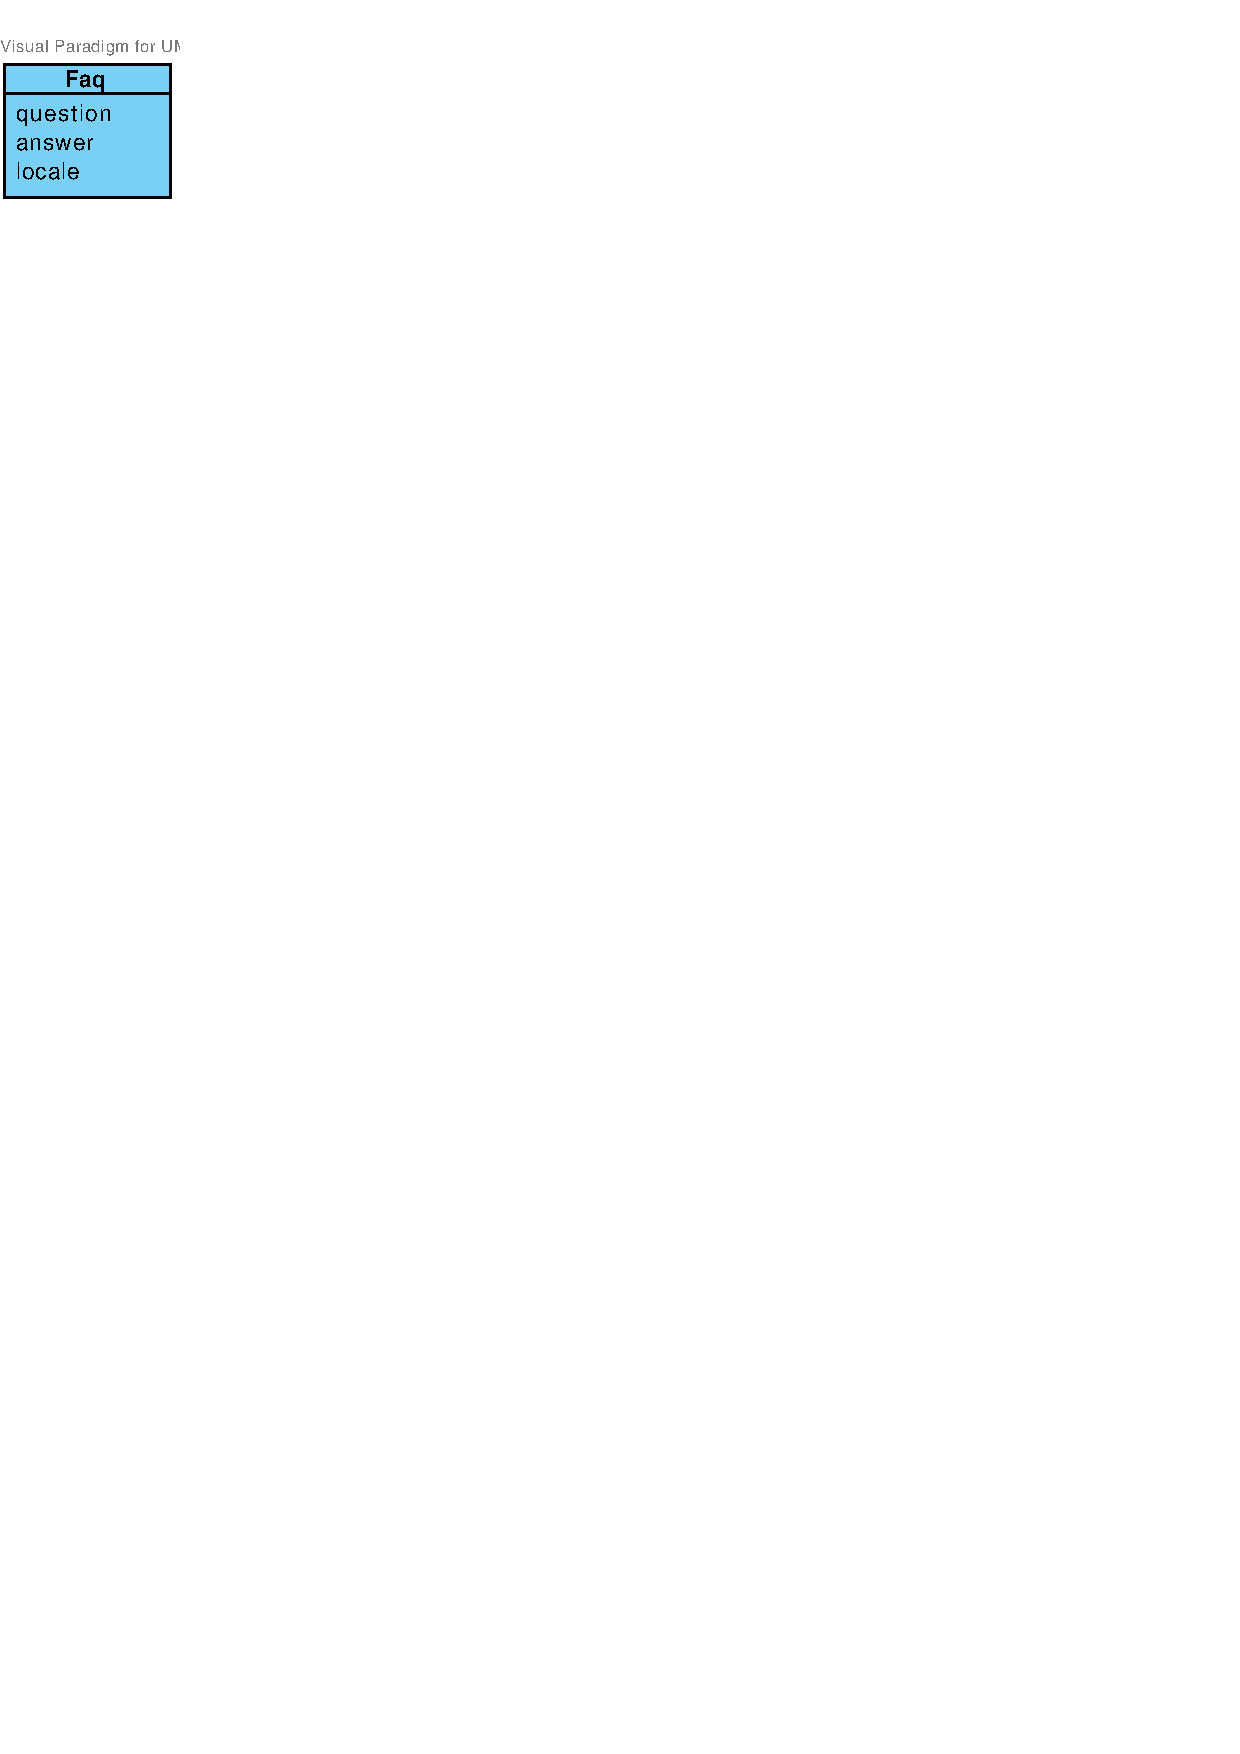
\includegraphics[trim=0 740 510 30, clip, keepaspectratio]{./images/domain-faq-entity.pdf}
    \caption{Model of \texttt{Faq} entity}
    \label{fig:domain-faq-entity}
\end{figure}

\section{Implementation}

The core project of this thesis is done by three students, therefore the implementation of it will be described in the thesis of student Jakub Cechacek.